%+----------------------------------------------------------------------------+
%| SLIDES: 
%| Chapter: Complementary material - details on Regular Reduction
%| Author: Casey Blacker
%+----------------------------------------------------------------------------+

%- HandOut Flag -----------------------------------------------------------------------------------------
\newif\ifHandout

%- D0cum3nt ----------------------------------------------------------------------------------------------
\documentclass[beamer,10pt]{standalone}   
%\documentclass[beamer,10pt,handout]{standalone}  \Handouttrue  

%- HandOut Flag -----------------------------------------------------------------------------------------
\ifHandout
	\setbeameroption{show notes} %print notes   
\fi

	
%- Packages ----------------------------------------------------------------------------------------------
\usepackage{custom-style}
\usepackage{math}
\usepackage[normalem]{ulem}

%--Beamer Style-----------------------------------------------------------------------------------------------
\usetheme{toninus}





%---------------------------------------------------------------------------------------------------------------------------------------------------
%- D0cum3nt ----------------------------------------------------------------------------------------------------------------------------------
\begin{document}
%------------------------------------------------------------------------------------------------

\begin{frame}
	\vfill
	
	{\centering \Huge EXTRA SLIDES on regular reduction}
	

	\vfill
	All the credit for the next slides is to C. Blacker

	\vspace{.5cm}\noindent
	\emph{Based on:}\\[1.5pt]
	B., Reduction of multisymplectic manifolds, \emph{Lett.\ Math.\ Phys.}, 2021

	\vspace{.5cm}\noindent
	\emph{See also:}\\[1.5pt]
	Reduction of multisymplectic manifolds \href{https://public.eimi.ru/~cblacker/Blacker.reduction\%20of\%20multisymplectic\%20manifolds.pdf}{(slides)} 
	at Good Morning SFARS, 7 June 2021.

\end{frame}



%------------------------------------------------------------------------------------------------
\begin{frame}\frametitle{The Problem of Multisymplectic Reduction}\label{frame:CaseySlides}
 \alert{Reduction is a procedure that takes a space and returns a ``smaller'' space}
 \vfill

	\begin{quotation}\noindent
		Reduction theory is by no means completed.\hspace{1.5pt}\textellipsis Only a few instances and examples of multisymplectic reduction are really well understood\textellipsis so one can expect to see more activity in this area as well.
	\end{quotation}
	--- J.\ Marsden and A.\ Weinstein, 2001, {\color{black!40}\emph{Comments on the history, theory, and applications of symplectic reduction}}

	\vspace{.8cm}

	\begin{quotation}\noindent
		One of the most interesting problems in multisymplectic geometry is how to extend the well-known Marsden--Weinstein reduction scheme for symplectic manifolds to the case of multisymplectic structures. 	
	\end{quotation}
	--- M.\ de Le\'on, 2018, {\color{black!40}\emph{Review of ``Remarks on multisymplectic reduction'' by Echeverr\'ia-Enr\'iquez, Mu\~noz-Lecanda, and Rom\'an-Roy}}
\end{frame}
%------------------------------------------------------------------------------------------------


%------------------------------------------------------------------------------------------------
\begin{frame}{The gist of: Symplectic Hamiltonian Actions \hfill\hyperlink{frame:symplecticmomaps}{\beamerreturnbutton{}}}\label{frame:gisthamaction}
	\center
	\vspace{-2pt}
	To specify a symplectic action ${\color{orange} G\curvearrowright M}$ \ldots

	\vspace{5pt}
	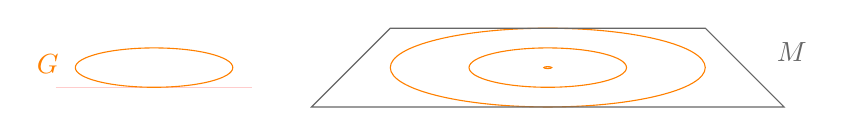
\begin{tikzpicture}
		\draw[red!20] (-6.25,.25) -- (-3.75,.25);
		\draw[orange] (-5,.5) ellipse (1 and .25);
		\node[orange] at (-6.35,.55) {$G$};

		\draw[orange] (0,.5) ellipse (.05 and .0125);
		\draw[orange] (0,.5) ellipse (1 and .25);
		\draw[orange] (0,.5) ellipse (2 and .5);
		\draw[black!60] (-3,0) -- (3,0) -- (2,1) -- (-2,1) -- cycle;
		\node[black!60] at (3.1,.7) {$M$};
	\end{tikzpicture}
	
	\vspace{5pt}
	\hspace{.75cm}we could describe the induced map ${\color{orange}\xi\mapsto\underline\xi}$ \ldots

	\vspace{5pt}
	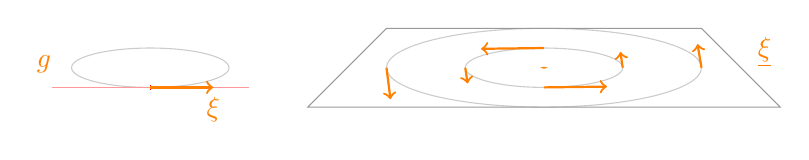
\begin{tikzpicture}
		\draw[black!20] (-5,.5) ellipse (1 and .25);
		\draw[red!40] (-6.25,.25) -- (-3.75,.25);
		\draw[red] (-5,.22) -- (-5,.28);
		\node[orange] at (-6.35,.55) {$\mathfrak{g}$};
		\draw[thick,orange,->] (-5,.25) -- (-4.2,.25) node[anchor=north] {$\xi$};

		\draw[black!20] (0,.5) ellipse (1 and .25);
		\draw[black!20] (0,.5) ellipse (2 and .5);
		\draw[black!40] (-3,0) -- (3,0) -- (2,1) -- (-2,1) -- cycle;

		\draw[orange,fill=red] (0,.5) ellipse (.02 and .02/4);

		\draw[thick,orange,->] (0,.25) -- (.8,.25+.01);
		\draw[thick,orange,->] (0,.75) -- (-.8,.75-.01);

		\draw[thick,orange,->] (1,.5) -- (.97,.7);
		\draw[thick,orange,->] (-1,.5) -- (-.97,.3);

		\draw[thick,orange,->] (2,.5) -- (2-.05,.8);
		\draw[thick,orange,->] (-2,.5) -- (-2+.05,.1);

		\node[orange] at (2.8,.7) {$\underline\xi$};
	\end{tikzpicture}

	\hspace{1.5cm} or an assignment of Hamiltonian functions ${\color{blue}\xi\mapsto f_{\underline\xi}}$.

	\vspace{5pt}
	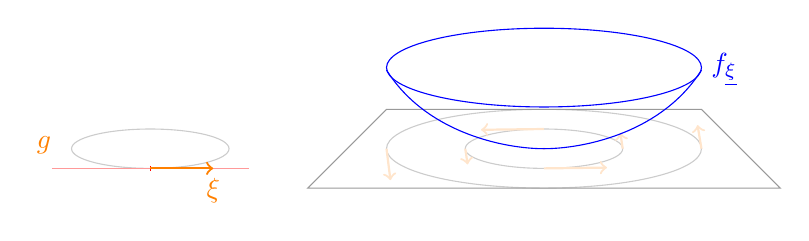
\begin{tikzpicture}
		\draw[black!20] (-5,.5) ellipse (1 and .25);
		\draw[red!40] (-6.25,.25) -- (-3.75,.25);
		\draw[red] (-5,.22) -- (-5,.28);
		\node[orange] at (-6.35,.55) {$\mathfrak{g}$};
		\draw[thick,orange,->] (-5,.25) -- (-4.2,.25) node[anchor=north] {$\xi$};

		\draw[black!20] (0,.5) ellipse (1 and .25);
		\draw[black!20] (0,.5) ellipse (2 and .5);
		\draw[black!40] (-3,0) -- (3,0) -- (2,1) -- (-2,1) -- cycle;

		\draw[red!20] (0,.5) ellipse (.02 and .02/4);

		\draw[thick,orange!20,->] (0,.25) -- (.8,.25+.01);
		\draw[thick,orange!20,->] (0,.75) -- (-.8,.75-.01);

		\draw[thick,orange!20,->] (1,.5) -- (.97,.7);
		\draw[thick,orange!20,->] (-1,.5) -- (-.97,.3);

		\draw[thick,orange!20,->] (2,.5) -- (2-.05,.8);
		\draw[thick,orange!20,->] (-2,.5) -- (-2+.05,.1);

		\draw[blue] (0,1.53) ellipse (2 and .5);

		\draw[blue] (0,.5) .. controls (.5,.5) and (1.5,.7) .. (2,1.5) node[anchor=west] {$f_{\underline\xi}$};
		\draw[blue] (0,.5) .. controls (-.5,.5) and (-1.5,.7) .. (-2,1.5);
	\end{tikzpicture}

	\vspace{-4pt}
	When this is possible\footnote{\color{black!50}\tiny{*and $\xi\mapsto f_{\underline\xi}$ is a homomorphism of Lie algebras}}, the action is called \textbf{Hamiltonian}.
	
\end{frame}
%------------------------------------------------------------------------------------------------

%------------------------------------------------------------------------------------------------
\begin{frame}\frametitle{Symplectic Reduction --- Idea}
	\[
		\omega = \underbrace{\;\d x_1\wedge\d y_1\;}_{\text{to be removed}}\hspace{3pt}+\hspace{5pt}  \d x_2\wedge\d y_2 + \cdots +\d x_n\wedge\d y_n
	\]

	\begin{center}
	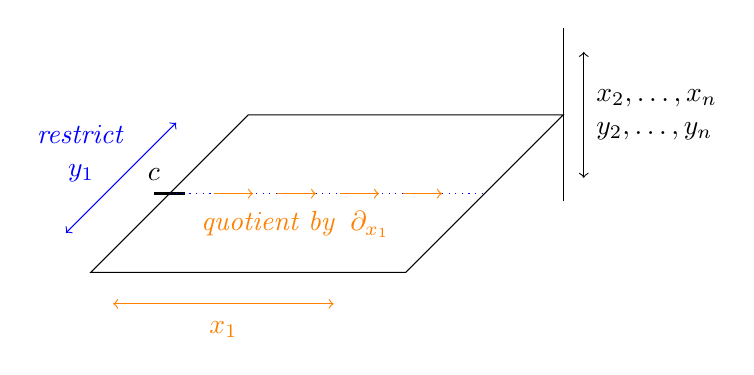
\begin{tikzpicture}[scale=2]	
		\draw (0,0) -- (2,0) -- (3,1) -- (1,1) -- cycle;
		\draw[<->,orange,xshift=-4.5pt] (.3,-.2) -- node[below=3pt,align=center] {$x_1$} (1.7,-.2);
		\draw[<->,blue,xshift=-4.5pt] (0,.25) -- node[above left=-5pt,align=center] {\emph{restrict}\\$y_1$} +(.7,.7);
		
		\draw[black,thick] (.5,.5) +(-.1,0) node[above=1pt] {$c$} -- +(.1,0);
		\draw[blue,dotted] (.5,.5) -- node[pos=.4,below=3pt,orange] {\emph{quotient by} \,$\partial_{x_1}$} (2.5,.5);

		\draw[orange,->] (.78,.5) -- +(.25,0);
		\draw[orange,->] (1.18,.5) -- +(.25,0);
		\draw[orange,->] (1.58,.5) -- +(.25,0);
		\draw[orange,->] (1.98,.5) -- +(.25,0);

		\draw (3,.45) -- (3,1.55);
		\draw[<->] (3.13,.6) -- node[right=1pt,align=left] {$x_2, \ldots ,x_n$\\$y_2, \ldots ,y_n$} (3.13,1.4);
	\end{tikzpicture}
	\end{center}
	
	\begin{center}
		\emph{{\color{blue}Restrict} and {\color{orange}quotient} conjugate degrees of freedom.}
	\end{center}
\end{frame}
%------------------------------------------------------------------------------------------------

%------------------------------------------------------------------------------------------------
\begin{frame}\frametitle{Symplectic Reduction --- Proof}
	\begin{center}
	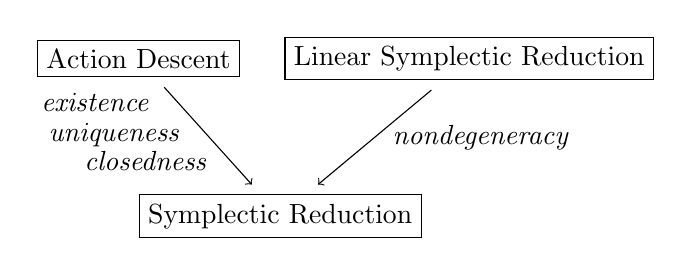
\begin{tikzpicture}
		\node (A) at (-2,2) {\fbox{Action Descent}};
		\node (B) at (2.2,2) {\fbox{Linear Symplectic Reduction}};
		\node (C) at (-.2,0) {\fbox{Symplectic Reduction}};

		\draw[->] (A)--(C);
		\draw[->] (B)-- node[right=3pt] {\emph{nondegeneracy}} (C);

		\node at (-2.54,1.44) {\emph{existence}};
		\node at (-2.3,1.03) {\emph{uniqueness}};
		\node at (-1.9,.7) {\emph{closedness}};
	\end{tikzpicture}
	\end{center}

	\vspace{-.3cm}
	\begin{enumerate}
		\item Apply the \emph{Action Descent Lemma} to $G_\lambda\curvearrowright\mu^{-1}(\lambda)$ and $i^*\omega$.
			\begin{center}
			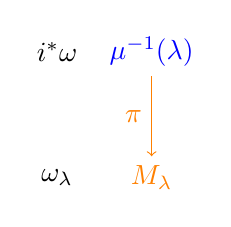
\begin{tikzpicture}[scale=2]
				\node[blue] (A) at (0,0) {$\mu^{-1}(\lambda)$};
				\node (A2) at (-.6,0) {$i^*\omega$};
				\node[orange] (C) at (0,-.8) {$M_\lambda$};
				\node (C2) at (-.6,-.8) {$\omega_\lambda$};

				\path[->,orange] (A) edge node[left] {$\pi$} (C);
			\end{tikzpicture}
			\end{center}

		\item Use \emph{Linear Symplectic Reduction} to conclude that $\omega_\lambda$ is nondegenerate.
	\end{enumerate}
\end{frame}
%------------------------------------------------------------------------------------------------

%------------------------------------------------------------------------------------------------
\begin{frame}\frametitle{The Action Descent Lemma}
	\begin{lemblock}
	If
	\begin{itemize}
		\item $G\curvearrowright M$ free and proper,
		\item $\alpha\in\Omega^*(M)$ \emph{invariant} and \emph{horizontal} ($\iota_{\underline\g}\hspace{1pt}\alpha=0$),
	\end{itemize}

	\vspace{-.3cm}
	\begin{center}
	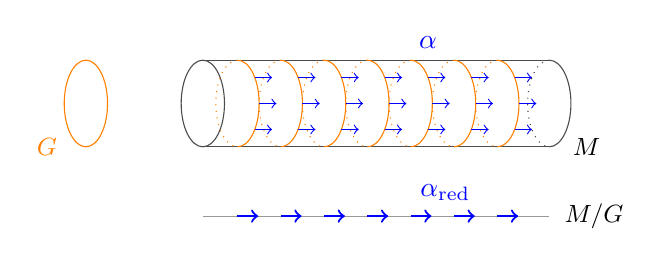
\begin{tikzpicture}[scale=1.1]
		\draw[yshift=-.8cm,black!40] (0,0) -- (4,0) node[black,right=2pt] {\small $M/G$};

		\begin{scope}[xshift=-1.35cm]
		\draw[orange] (0,.5) ellipse (.25 and .5);
		\end{scope}

		\node[orange] at (-1.8,0) {\small $G$};

		\node[orange] at (-.7,.5) {$\curvearrowright$};

		\draw[black!70] (0,.5) ellipse (.25 and .5);
		\draw[black!70] (4,0) arc (-90:90:.25 and .5);
		\draw[dotted,black!70] (4,1) arc (90:270:.25 and .5);
		\draw[black!70] (0,0) -- (4,0) node[black,right=5pt] {\small $M$};
		\draw[black!70] (0,1) -- (4,1);

		\foreach \x in {-1,-.5,...,2}
		{
			\begin{scope}[xshift=\x cm]
				\draw[orange,xshift=1.4cm] (0,0) arc (-90:90:.25 and .5);
				\draw[orange,dotted,xshift=1.4cm] (0,1) arc (90:270:.25 and .5);

				\draw[blue,->,shift={(1.7,.2)}] (-.1,0) -- (.1,0);
				\draw[blue,->,shift={(1.7,.8)}] (-.1,0) -- (.1,0);
				\draw[blue,->,shift={(1.75,.5)}] (-.1,0) -- (.1,0);
			\end{scope}

			\begin{scope}[xshift=\x cm]
				\draw[blue,->,thick,shift={(1.5,-.8)}] (-.1,0) -- (.14,0);
			\end{scope}
		}

		\node[blue] at (2.6,1.2) {$\alpha$};
		\node[blue] at (2.8,-.53) {$\alpha_{\mathrm{red}}$};
	\end{tikzpicture}
	\end{center}
	\vspace{-.4cm}
	then
	\begin{itemize}
		\item $\exists ! \,\alpha_{\mathrm{red}}\in\Omega^*(M/G)$ such that $\alpha=\pi^*\alpha_{\mathrm{red}}$,
		\item $\d\alpha=0 \implies \d\alpha_{\mathrm{red}}=0$.
	\end{itemize}
	\end{lemblock}	

\end{frame}
%------------------------------------------------------------------------------------------------



%------------------------------------------------------------------------------------------------
\begin{frame}\frametitle{The Space of Moment Maps}
	\vspace{-.2cm}
	\begin{itemize}
		\item $(M,\omega,G,\mu)$ Hamiltonian $G$-space
		\item $\phi\in\Omega^{k-1}(M,\g^*)$
	\end{itemize}

	\vspace{.3cm}
	\emph{Question:} When is $\mu+\phi$ a moment map?
	\vspace{.3cm}

	\begin{itemize}
		\item ${\color{green}\d\phi=0}$, since
			\[
				\d(\mu+\phi)_\xi = \iota_\xi\omega \iff \d\phi_\xi=0.
			\]
		\item ${\color{green}\L_\xi\phi_\zeta=\phi_{[\xi,\zeta]}}$, as
			\[
				\L_\xi (\mu+\phi) = (\mu+\phi)_{[\xi,\zeta]} \iff \L_\xi\phi = \phi_{[\xi,\zeta]}.
			\]
	\end{itemize}
	
	\vspace{.2cm}
	i.e.\ $\phi$ is a moment map for the trivial action $G\curvearrowright M$.

	\vspace{.2cm}
	{\tiny The space of moment maps is an affine space modeled on $\{\phi\in\Omega^{k-1}(M,\g^*)\,|\,\d\phi=0,\;G_\phi=G\}$.}
\end{frame}

\begin{frame}\frametitle{The Leibniz Condition and the Induced Action on Forms}
	\vspace{-.2cm}
	\begin{itemize}
		\item $\phi\in\Omega^*(M,\g^*)$
		\item $\xi\in\g$
	\end{itemize}

	\vspace{-.4cm}
	\begin{align*}
		{\color{black!40}\forall\zeta\in\g:\hspace{.3cm}}\L_\xi\phi_\zeta=\phi_{[\xi,\zeta]}	&&{\color{black!40}\iff\forall\zeta\in\g:}
					&&0	&=	\L_\xi\phi_\zeta - \phi_{[\xi,\zeta]}			\\
					&&						&&	&=	\L_\xi\phi_\zeta + \langle\mathrm{ad}_\xi^*\phi,\zeta\rangle\\
					&&						&&	&=	\langle\L_\xi\phi + \mathrm{ad}_\xi^*\phi,\zeta\rangle	\\
					&&						&&	&	\\[-8pt]
					&&	{\color{black!40}\iff}\hspace{.3cm}	&&0	&=	(\L_\xi + \mathrm{ad}_\xi^*)\hspace{2pt}\phi					\\
					&&						&&	&	\\[-8pt]
					&&	{\color{black!40}\iff}\hspace{.3cm}	&&\xi	&\in	\g_\phi
	\end{align*}
	in terms of the induced action $G\curvearrowright\Omega^*(M,\g^*)$. Thus,
	\[
		{\color{black!40}\forall\xi,\zeta\in\g:\hspace{.3cm}}\L_\xi\phi_\zeta=\phi_{[\xi,\zeta]}	\hspace{.3cm}{\color{black!40}\iff}\hspace{.3cm}	G\cdot\phi = \phi
	\]
\end{frame}

\begin{frame}\frametitle{Level Sets of the Moment Map}
	Rather than:
	\begin{itemize}
		\item {\color{green}family of moment maps} $\{\mu-\phi\,|\,\d\phi=0,\;G_\phi=G\}$
		\item reduction at $\mu-\phi=0$
	\end{itemize}


	\vspace{.5cm}
	We instead consider:
	\begin{itemize}
		\item fixed moment map $\mu$
		\item {\color{green}family of levels} $\{\phi\,|\,\d\phi=0,\;\text{\sout{$G_\phi=G$}}\}$
		\item reduction at $\mu=\phi$
	\end{itemize}

	\vspace{.5cm}
	%The \emph{level set} associated to $\phi$ is
	\emph{$\phi$-level set:}
	\[
		\mu^{-1}(\phi) := \{\mu=\phi\}
	\]
\end{frame}


%%%%% MULTISYMPLECTIC REDUCTION

\begin{frame}\frametitle{Multisymplectic Reduction --- Proof Idea}
	\begin{center}
	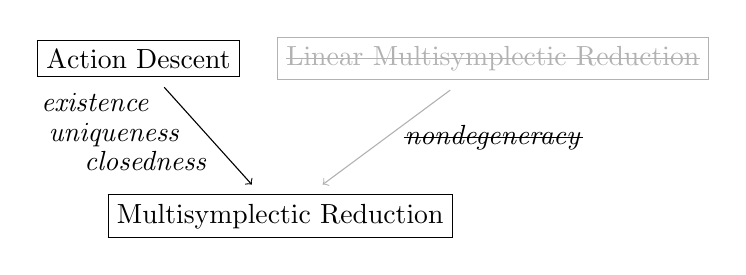
\begin{tikzpicture}
		\node (A) at (-2,2) {\fbox{Action Descent}};
		\node[black!30] (B) at (2.5,2) {\fbox{\sout{Linear Multisymplectic Reduction}}};
		\node (C) at (-.2,0) {\fbox{Multisymplectic Reduction}};

		\draw[->] (A)--(C);
		\draw[->,black!30] (B)-- node[right=3pt,black] {\sout{\emph{nondegeneracy}}} (C);

		\node at (-2.54,1.44) {\emph{existence}};
		\node at (-2.3,1.03) {\emph{uniqueness}};
		\node at (-1.9,.7) {\emph{closedness}};
	\end{tikzpicture}
	\end{center}

	\vspace{-.3cm}
	\begin{enumerate}
		\item Apply the \emph{Action Descent Lemma} to $G_\phi\curvearrowright\mu^{-1}(\phi)$ and $i^*\omega$.
			\begin{center}
			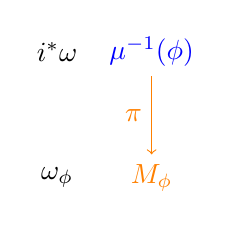
\begin{tikzpicture}[scale=2]
				\node[blue] (A) at (0,0) {$\mu^{-1}(\phi)$};
				\node (A2) at (-.6,0) {$i^*\omega$};
				\node[orange] (C) at (0,-.8) {$M_\phi$};
				\node (C2) at (-.6,-.8) {$\omega_\phi$};

				\path[->,orange] (A) edge node[left] {$\pi$} (C);
			\end{tikzpicture}
			\end{center}

		\item {\color{black!30}\sout{Use \emph{Linear Multisymplectic Reduction} to conclude that $\omega_\phi$ is nondegenerate.}}
	\end{enumerate}
\end{frame}

\begin{frame}\frametitle{Multisymplectic Reduction --- Proof Outline}
	Two steps:
	\begin{enumerate}
		\item ${\color{orange}G_\phi\curvearrowright M}$ preserves ${\color{blue}\mu^{-1}(\phi)}$,
		\item $i^*\omega$ is invariant and horizontal.
	\end{enumerate}
\end{frame}

\begin{frame}\frametitle{Multisymplectic Reduction --- Proof (Step 1)}
	\begin{enumerate}
		\item {\color{orange}$G_\phi\curvearrowright M$} preserves {\color{blue}$\mu^{-1}(\phi)$}.
	\end{enumerate}

	\vspace{.4cm}
	\begin{itemize}
		\item $\mu^{-1}(\phi) = \{\mu-\phi=0\}$

		\vspace{.4cm}
		\item {\color{black}$\forall\,\xi,\zeta\in\g_\phi$,}
			\vspace{-.2cm}
			\begin{align*}
				\L_\xi\hspace{1pt} (\mu-\phi)_\zeta
					&=	(\mu-\phi)_{[\xi,\zeta]},	&&\hspace{-.2cm}\text{by the Leibniz condition,}	\\
					&=	0				&&\hspace{-.2cm}\text{on $\mu^{-1}(\phi)$.}
			\end{align*}
	\end{itemize}
\end{frame}

\begin{frame}\frametitle{Multisymplectic Reduction --- Proof (Step 2)}
	\begin{enumerate}\setcounter{enumi}{1}
		\item $i^*\omega$ is invariant and horizontal.
	\end{enumerate}

	\vspace{.2cm}

	\begin{itemize}
		\item \textbf{invariant:} Hamiltonian actions are multisymplectic.\\[3pt]
		\item \textbf{horizontal:} For $\xi\in\g_\phi$,
		\begin{align*}
			\iota_\xi i^*\omega
				&=	i^* {\color{red}\iota_\xi\omega},	&&\hspace{-1cm}\text{since ${\color{orange}G_\phi}$ preserves ${\color{blue}\mu^{-1}(\phi)}$,}		\\
				&=	i^* {\color{red}\d\mu_\xi},	&&\hspace{-1cm}\text{by the Hamiltonian condition,}	\\
				&=	i^* \d\phi_\xi,			&&\hspace{-1cm}\text{since ${\color{blue}\mu=\phi}$ on ${\color{blue}\mu^{-1}(\phi)}$,}		\\
				&=	0,					&&\hspace{-1cm}\text{as ${\color{blue}\phi}$ is closed.}
		\end{align*}
	\end{itemize}
	\hspace*{\fill}$\qed$
\end{frame}


%%%%%  REDUCTION OF CLOSED FORMS

\begin{frame}\frametitle{Extension: Reduction of Closed Forms}
	\begin{enumerate}
		\item The proof makes no use of the nondegeneracy or homogeneity of $\omega\in\Omega^{k+1}(M)$.
		\item Extends naturally to a reduction scheme for closed forms.
	\end{enumerate}

	\vspace{-.3cm}
	\begin{align*}
		\omega	&\in\Omega^*(M) \text{ closed}		\\
		\phi	&\in\Omega^*(M,\g^*) \text{ closed}
	\end{align*}

	\vspace{-.4cm}
	\begin{align*}
				&\hspace{-.8cm}\underline{\mu\in\Omega^*(M,\g^*)}	\\
		\d\mu_\xi	&=	\iota_\xi\omega					\\
		\L_\xi\mu_\zeta	&=	\mu_{[\xi,\zeta]}
	\end{align*}
\end{frame}
%------------------------------------------------------------------------------------------------


%------------------------------------------------------------------------------------------------
\end{document}
